
%(BEGIN_QUESTION)
% Copyright 2010, Tony R. Kuphaldt, released under the Creative Commons Attribution License (v 1.0)
% This means you may do almost anything with this work of mine, so long as you give me proper credit

Suppose you are summoned to diagnose a process control problem, and are shown this trend graph of the PV, SP, and Output for a particular loop:

$$\includegraphics[width=15.5cm]{i01388x01.eps}$$

We see the process variable clearly deviating from setpoint, which it should not do if the control system is doing its job as it should.

\vskip 10pt

Determine the most likely cause of the problem, based on the data you see in this trend.

\vskip 20pt \vbox{\hrule \hbox{\strut \vrule{} {\bf Suggestions for Socratic discussion} \vrule} \hrule}

\begin{itemize}
\item{} Explain why viewing the {\it output} trend in addition to the PV trend is critically important to being able to diagnose the problem here.
\item{} Examine this trend graph and explain how we can tell which mode ({\it automatic} or {\it manual}) the loop controller is in.
\item{} Examine this trend graph and explain how we can tell which direction of action ({\it direct} or {\it reverse}) the loop controller is configured for.
\item{} Identify as best you can the {\it proportional band} and {\it bias} values of this controller based on the data shown in the trend.
\item{} Suppose the control valve in a process loop were to fail shut and thereby become unresponsive to the controller's output signal.  How do you think this would affect the trend graph of PV, SP, and Output for the loop?  
\item{} Suppose the paper chart recorder displaying this trend graph were to fail in such a way that the PV pen drops all the way down to zero and becomes unresponsive to the transmitter's signal.  Could an operator extrapolate the value of the PV just by examining the SP and Output trends?  Explain why or why not.
\end{itemize}

\underbar{file i01388}
%(END_QUESTION)





%(BEGIN_ANSWER)

The problem is most likely the controller, but I will let you determine the nature of the problem!

%(END_ANSWER)





%(BEGIN_NOTES)

This controller's tuning is clearly not aggressive enough to handle the loads in this process.  We see the output signal hardly varying at all as the PV deviates substantially -- and for great lengths of time -- from setpoint.  The movements in output signal are clearly not enough to have significant effect on the PV.

\vskip 10pt

A change we could make to improve the quality of control is to increase the controller's gain, so that any change in PV will result in a greater change (more aggressive response) in the output signal.

%INDEX% Process troubleshooting: diagnosing problem via trend recording

%(END_NOTES)


